\chapter {Marco teórico}
 \section{Sistemas de recomendación}
 	Frecuentemente es necesario hacer elecciones sin tener la suficiente experiencia personal o conocimiento sobre las atternativas existentes. En la vida diaria, se confía en las recomendaciones que otras personas hacen de palabra, cartas de recomendación, reseñas de libros, películas o encuestas generales. \cite{4}
 	Los sistemas de recomendación asisten y aumentan este proceso social. En un sistema de recomendación típico la gente provee de información como entradas que sirven para dar sugerencias y cabe destacar que se diferencía de un motor de búsqueda por la razón de individualidad que se pretende brindar al tener un sistema personalizado, ya que el criterio de qué tan relevante o útil pueda ser un artículo varía para cada usuario y no es general para todos. Estas diferencias generan distintas aproximaciones en el comportamiento de un sistema de recomendación, donde la tendencia es combinar distintas técnicas de recomendación para mejorar el desempeño del sistema. Las técnicas de recomendación tienen distintas clasificaciones dependiendo de las fuentes de datos en las que se basa la recomendación y el uso en que la información es puesta. Especificamente, los sistemas de recomendación tienen (i) información previa, la información que el sistema tiene antes de que se realice la recomendación; (ii) información de entrada, la información que el usuario debe comunicar al sistema para generar una recomendación, y (iii) un algoritmo que combina la información previa y la recibida del usuario para mostrar sus sugerencias. Con esta base, es posible identificar diferentes técnicas.% como se puede observar en la tabla~\ref{table:tecnicas de recomendacion}.

 	\subsection{Técnicas de recomendación}
	 	La recomendación \emph{colaborativa} es probablemente la más familiar, mayormente implementada y más madura de las tecnologías. Los sistemas de recomendación colaborativos agregan \it{ratings} (evaluaciones) a los objetos, reconocen la similitud entre los usuarios de acuerdo a sus \it{ratings} y generan recomendaciones con base en las comparaciones entre usuarios.
	 	Las recomendaciones \emph{demográficas} pretenden categorizar al usuario con base en sus atributos personales y hacer recomendaciones de acuerdo a clases demográficas. La representación de la información demográfica en el modelo puede variar enormemente, dependiendo de las necesidades del sistema y de la información que pueda recabar. Las técnicas de recomendación demográficas también utilizan algún tipo de correlación entre los usuarios, pero difieren de las colaborativas en medida de que no requieren de la interacción explícita de los ratings para obtener recomendaciones. 
	 	Las recomendaciones \emph{basadas en contenido} representan la continuación y crecimiento de las investigaciones sobre filtrado de datos. En un sistema de recomendación basado en contenido, los objetos de interés son definidos por sus características que pueden ser asociadas entre varios objetos. El sistema basado en contenido utiliza la información de los objetos para categorizarlos a través de una correlación entre los objetos y entonces, con base en la interacción del usuario, recomendar objetos similares a aquellos con los que ha interactuado. Los perfiles de usuarios dependen del método de aprendizaje empleado. Han sido usados árboles de decisión, redes neuronales y representaciones basadas en vectores por igual. Este tipo de modelos son de larga duración y solo son actualizados mientras el usuario tiene mayor interacción con los mismos.
	 	Por el contrario, las recomendaciones \emph{por utilidad} y \emph{basadas en conocimiento} no pretenden dar soluciones generales a largo plazo sobre sus usuarios, sino que se basan en la evaluación entre la necesidad actual del usuario y el set de opciones disponible. Las recomendaciones basadas en utilidad hacen sugerencias con base en el cómputo de la utilidad que tiene el usuario para cada objeto. Por supuesto, el problema central es como crear una función de utilidad para cada usuario. El beneficio de las recomendaciones basadas en utilidad es que permiten factorizar atributos, haciendo posible elevar la importancia de una característica frente a otra. 
	 	Los sistemas \emph{basados en conocimiento} pretenden sugerir objetos basados en inferencias acerca de las necesidades del usuario y preferencias. En cierto sentido, se puede decir que todas las técnicas de recomendación hacen algún tipo de inferencia, pero los sistemas basados en conocimiento se distinguen porque tienen conocimiento funcional, de como un artículo en particular puede empatar una necesidad de usuario. El modelo para el perfil de usuario puede ser cualquier estructura de conocimiento que permita la inferencia. \cite{5}

 	\subsection{Comparando técnicas de recomendación}
 		Todas las técnicas de recomendación tienen sus fortalezas y sus debilidades, quizás el más conocido es el problema de \it{cold start}, que sucede tanto para usuarios como para objetos. Ya que al tener un usuario nuevo, es difícil categorizarle debido a la poca o nula interacción que ha tenido con el sistema. De la misma manera, cuando un objeto es nuevo, no tiene muchas evaluaciones de usuarios y no puede ser recomendado tan fácilmente. Entre estos, las principales ventajas y desventajas de las técnicas de recomendación mencionadas pueden ser visualizadas en la tabla~\ref{table: comparando tecnicas de recomendacion}\cite{5}
 		
 		\clearpage
 		\begin{table}[h]
		\begin{center}
		 \begin{tabular}{| c | c | c |}
		 \toprule
		 	\textbf{Técnica} & \textbf{Fortalezas} & \textbf{Debilidades}\\
		 \midrule
		 	Filtrado colaborativo & 
		 	\parbox{5cm}{\begin{itemize}[topsep=0pt]
		 		\item Puede identificar nichos cruzados
		 		\item No necesita dominio de conocimiento
		 		\item Adaptativo: la calidad mejora sobre el tiempo
		 		\item Retroalimentación implícita suficiente
		 	\end{itemize}} &
		 	\parbox{5cm}{\begin{itemize}[topsep=0pt]
		 		\item Problema \i{ramp-up} con los usuarios nuevos
		 		\item Problema \i{ramp-up} con los objetos nuevos
		 		\item Problema de la oveja gris (problemas con clasificaciones que no pertenecen en concreto a un nicho)
		 		\item La calidad depende de grandes volúmenes de históricos.
		 		\item El problema de la plasticidad contra la estabilidad.
		 	\end{itemize}} \\
		 \midrule
		 	Basado en contenido & 
		 	\parbox{5cm}{\begin{itemize}[topsep=0pt]
		 		\item No necesita dominio de conocimiento
		 		\item Adaptativo: la calidad mejora sobre el tiempo
		 		\item Retroalimentación implícita suficiente
		 	\end{itemize}} &
		 	\parbox{5cm}{\begin{itemize}[topsep=0pt]
		 		\item Problema \i{ramp-up} con los usuarios nuevos
		 		\item La calidad depende de grandes volúmenes de históricos.
		 		\item El problema de la plasticidad contra la estabilidad.
		 	\end{itemize}} \\
		 \midrule
		 	Filtrado demográfico & 
		 	\parbox{5cm}{\begin{itemize}[topsep=0pt]
		 		\item Puede identificar nichos cruzados
		 		\item No necesita dominio de conocimiento
		 		\item Adaptativo: la calidad mejora sobre el tiempo
		 	\end{itemize}} &
		 	\parbox{5cm}{\begin{itemize}[topsep=0pt]
		 		\item Problema \i{ramp-up} con los usuarios nuevos
		 		\item Problema de la oveja gris (problemas con clasificaciones que no pertenecen en concreto a un nicho)
		 		\item La calidad depende de grandes volúmenes de históricos.
		 		\item El problema de la plasticidad contra la estabilidad.
		 		\item Debe obtener información demográfica sensible.
		 	\end{itemize}} \\
		 \bottomrule
			\end{tabular}
	 	\end{center}
		\end{table}
		\begin{table}[h]
		\begin{center}
		 \begin{tabular}{| c | c | c |}
		 \toprule
		 	\textbf{Técnica} & \textbf{Fortalezas} & \textbf{Debilidades}\\
		 \midrule
		 	Basado en utilidad & \parbox{5cm}{\begin{itemize}[topsep=0pt]
		 		\item No requiere curva de aprendizaje (\i{ramp-up})
		 		\item Sensible a los cambios en las preferencias
		 		\item Puede incluir características que no son de los productos
		 	\end{itemize}} &
		 	\parbox{5cm}{\begin{itemize}[topsep=0pt]
		 		\item El usuario debe introducir la función de utilidad
		 		\item Habilidad de sugerencia estática (no aprende)
		 	\end{itemize}} \\
		 \midrule
		 	Basado en conocimiento & 
		 	\parbox{5cm}{\begin{itemize}[topsep=0pt]
		 		\item No requiere curva de aprendizaje (\i{ramp-up})
		 		\item Sensible a los cambios en las preferencias
		 		\item Puede incluir características que no son de los productos
		 		\item Puede mapear de necesidad de usuario a productos
		 	\end{itemize}} &
		 	\parbox{5cm}{\begin{itemize}[topsep=0pt]
		 		\item Habilidad de sugerencia estática (no aprende)
		 		\item Requiere ingeniería de conocimiento.
		 	\end{itemize}} \\
		 \bottomrule
			\end{tabular}
		 \caption{Comparación de las distintas técnicas de recomendación}
	 	 \label{table: comparando tecnicas de recomendacion}
	 	\end{center}
		\end{table}

	\subsection{Sistemas híbridos}
		Con el fin de obtener un mejor desempeño en los sistemas de recomendación, se utilizan al mismo tiempo dos o más de las técnicas descritas previamente para formar lo que se denomina un sistema híbrido, donde estás diferentes técnicas pueden convivir de maneras diferentes como se puede visualizar en la tabla~\ref{table: sistemas hibridos}

		\clearpage
		\begin{table}[h]
		\begin{center}
		 \begin{tabular}{| c | p{10cm} |}
		 \toprule
		 	\textbf{Método de hibridización} & \textbf{Descripción} \\
		 \midrule
		 	Ponderado & Las evaluaciones (o votos) de distintas técnicas de recomendación son combinadas juntas para producir una sola recomendación.\\
		 \midrule
		 	Switching & El sistema intercambia entre técnicas de recomendación dependiendo de la situación.\\
		 \midrule
		 	Mezclado & Recomendaciones de diferentes técnicas son presentadas al mismo tiempo.\\
		 \midrule
		 	Combinación de características & Características de distintas fuentes de información son utilizadas juntas en un solo algoritmo de recomendación\\
		 \midrule
		 	Cascada & Una técnica de recomendación refina las recomendaciones dadas por otra. \\
		 \midrule
		 	Aumento de funcionalidad & La salida de una técnica es usada como entrada de otra.\\
		 \midrule
		 	Nivel-meta & El modelo aprendido por un recomendador es usado como entrada de otro.\\
		 \bottomrule
			\end{tabular}
		 \caption{Sistemas híbridos}
	 	 \label{table: sistemas hibridos}
	 	\end{center}
		\end{table}\cite{5}

\newpage
 \section{Algoritmos de recomendación}
 \subsection{Vecinos próximos (k-NN)}
 	 Este método selecciona los k vecinos más similares al usuario o al ítem objetivo, de forma que mediante la combinación lineal del rating de los vecinos se realiza una predicción de rating. A partir de esta predicción, podemos sacar el ránking de ítems a recomendar, simplemente ordenándolos por orden descendente del rating predicho. Existe una gran cantidad de variaciones para estos algoritmos, ya que tienen muchos parámetros configurables que dan diferentes resultados dependiendo de los datos con los que se traten. El número k de vecinos, la similitud mínima a considerar como relevante, o el número de ítems en común para una similitud válida son algunos de los parámetros a establecer para estos algoritmos. Los algoritmos de vecinos próximos se han desarrollado en dos perspectivas posibles: recomendación de vecinos próximos por usuario y por ítem.
 	 \subsubsection{Basado en usuario}
 	 	Se recomiendan al usuario los ítems que han gustado a usuarios similares a éste. Su fórmula es la siguiente: \\
 	 	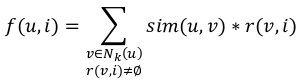
\includegraphics[width=0.4\textwidth]{images/knn_user}

 	 \subsubsection{Basado en item}
 	 	Se recomiendan al usuario los ítems que se parecen a ítems que le han gustado. Su función es muy similar a la del algoritmo k-NN con usuarios.\\
 	 	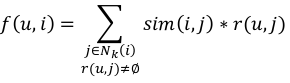
\includegraphics[width=0.4\textwidth]{images/knn_item}
 	 
 	 Normalmente, este algoritmo se utiliza con el número de vecinos igual al número total de ítems, es decir, que el vecindario de cada ítem son todos los demás existentes en el conjunto de datos. En cuanto a la función de similitud entre los usuarios o ítems, ésta se puede realizar mediante varios métodos, entre ellos destacan: 
 	 \begin{itemize}
 	 	\item \textbf{Coseno:} Mide el ángulo entre los vectores (ratings) década par de usuarios o ítems, de forma que son más similares aquellos cuyos vectores tienen la misma orientación. \\
 	 	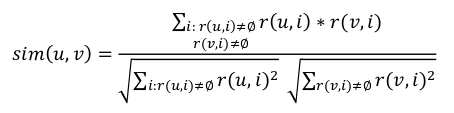
\includegraphics[width=0.7\textwidth]{images/coseno}

 	 	\item \textbf{Jaccard:} Dos usuarios o ítems son más similares cuanto más parecida sea la intersección a la unión de ambos, es decir, cuantos más ratings en común tengan, independientemente del valor de rating. \\
 	 	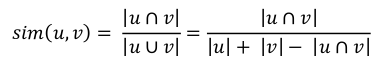
\includegraphics[width=0.5\textwidth]{images/jaccard}

 	 	\item \textbf{Pearson:} Equivalente a la similitud por coseno, pero cada rating se centra en la puntuación promedio del usuario (o ítem) correspondiente. Para este caso existen dos versiones dependiendo de la forma de calcular el módulo de v: por intersección, donde se suman los ratings de los ítems que tiene en común con u;y total, donde también se incluyen los ratings de aquellos que u desconoce. \\
 	 	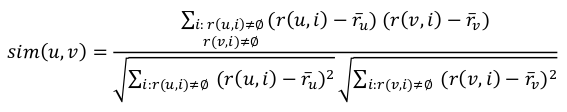
\includegraphics[width=0.8\textwidth]{images/pearson}

 	 \end{itemize}

 	\subsection{Slope One}
	El filtrado colaborativo es una técnica usada por los Sistemas de Recomendación para combinar las opiniones y pruebas de diferentes usuarios con el fin de obtener recomendaciones personalizadas. Hay al menos dos clases de filtrados colaborativos: las técnicas basadas en usuarios son derivadas de la medición de similitudes entre usuarios, mientras que las técnicas basadas en artículos comparan las valoraciones dadas por distintos usuarios. Slope One es una familia de algoritmos usados para el Filtrado Colaborativo introducida en Slope One Predictors for Online Rating-Based Collaborative Filtering por Daniel Lemire y Anna Maclachlan. Posiblemente, esta es la forma más simple de filtrado colaborativo basado en artículos. Su simplicidad la hace especialmente sencilla de implementar eficientemente mientras que su exactitud está a la par de algoritmos más complejos y costosos.
 	
 	\subsection{Factorización de matrices}
 		A los gustos de los usuarios y las características de los ítems subyace un espacio no visible que realmente determina por qué les gustan los ítems. Hay formalismos matemáticos que nos permiten hacer aflorar este tipo de espacio latente como unas cuantas dimensiones reducidas, sin tener que concretar qué son realmente esas dimensiones, y pudiendo sin embargo generar recomendaciones operando con ellas. La idea es representar tanto los ítems como los usuarios como vectores en un espacio de factores latentes, con una coordenada por factor que representa el grado de afinidad del usuario (o del ítem) hacia ese factor.Este efecto se puede realizar mediante la factorización de matrices representada en la figura~\ref{fig: matrix factorization}, descomponiendo la matriz original de ratings en un producto de varias matrices, dos o tres dependiendo del algoritmo, obteniendo siempre una primera matriz de usuarios por factores y una última de factores por ítems.

 		\begin{figure}[h!]
		 \centering
		 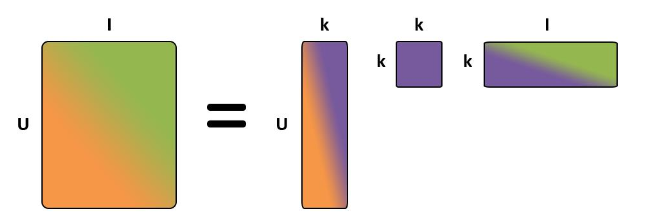
\includegraphics[width=12cm]{./images/matrix_fact}
		 \caption{Descomposición de la matrix en el producto de otras tres}
		 \label{fig: matrix factorization}
		\end{figure}

 		De esta forma, se obtienen k factores latentes que establecen un espacio de características común, tanto para los usuarios como para los ítems, permitiendo la comparación directa entre ellos.Así, un usuario da ratings de acuerdo a sus factores latentes y a los factores latentes del ítem.
 		A partir de aquí se ha desarrollado en el área gran cantidad de algoritmos para obtener la factorización de matrices, entre los que destacamos los siguientes:

 		\textbf{pLSA(probabilistic Latent Semantic Analysis):} Divide la matriz de ratings en dos, usuarios por factores y factores por ítems, de forma que su función de ránking equivale a la probabilidad de que el usuario puntúe al ítem según el espacio de factores latentes.\\
 		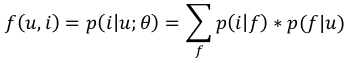
\includegraphics[width=0.5\textwidth]{images/plsa}

		\textbf{SVD(Singular Value Decomposition):} La factorización de la matriz de ratings genera tres matrices, para lo que se tiene en cuenta todos los ratings, asignándoles un cero a aquellos no conocidos. Se obtienen los vectores de usuario e ítem mediante el producto de las matrices obtenidas según la fórmula que se indica a continuación, de forma que su función de ránking consiste en la multiplicación de los vectores de usuario e ítem,centrado en la media del usuario.\\
		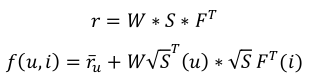
\includegraphics[width=0.5\textwidth]{images/svd}

		\textbf{SVDN(SVD no-empty entries):} Variante del anterior algoritmo en la que se obtienen dos matrices en lugar de tres,se tiene en cuenta únicamente los ratings conocidos, y su función de ránking no se centra en la media del usuario.\\
		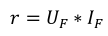
\includegraphics[width=0.2\textwidth]{images/svdn1}

		En este caso, entonces, el cálculo de dicha función es más inmediato, ya que los vectores de usuario e ítem se corresponden con la fila de la primera matriz y la columna de la segunda respectivamente, por lo que únicamente se multiplican la fila por la columna correspondiente.\\
		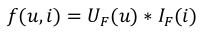
\includegraphics[width=0.4\textwidth]{images/svdn2}

		\textbf{HSVD(SVD with Hypergraph transformation):} Este método está dirigido a la recomendación de ítems a usuarios nuevos en el sistema, es decir, con poca actividad en el entrenamiento. Por ello, el primer paso del algoritmo consiste en dividir la matriz de ratings en tres: ratings de los usuarios que no están en test, ratings conocidos (de entrenamiento) de los usuarios que están en test, y ratings desconocidos de los usuarios que están en test (lo que se recomendará).

		\textbf{ASVD(Assymetric SVD):} Se trata de la versión asimétrica de SVD, que solo usa la tercera matriz de la descomposición para realizar las recomendaciones.Sigue exactamente los mismos pasos que HSVD, con la diferencia de que no se binariza la matriz de ratings de los usuarios viejos, sino que se utiliza la original con los ratings numéricos.

		\subsection{Basados en contenido}
		Este grupo de algoritmos se basa en la utilización de la descripción o características de cada ítem para realizar sugerencias sin utilizar información de otros usuarios para generar la recomendación. Destacan los algoritmos Rocchio y la implementación del k-NN para este tipo de sistemas de recomendación.
.
		\textbf{Rocchio:} Se basa en el cálculo de centroides para cada usuario, de forma que se obtenga un vector representante para cada uno. Estas clases se corresponderán con las características de los ítems, por ejemplo, en Twitter, las palabras clave del contenido de los tweets. De esta forma, se obtiene para cada usuario un centroide que representa su relación con cada característica. La fórmula para el cálculo de los centroides es la siguiente:\\
		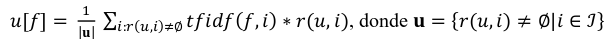
\includegraphics[width=\textwidth]{images/rocchio}
		Una vez se dispone de los centroides, el cálculo de la similitud de los usuarios con cada uno de los ítems se realiza mediante cualquiera de los métodos anteriormente descritos. 

		\textbf{k-NN (ítems):} Para la implementación del k-NN, la estructura de este algoritmo es idéntica a la de filtrado colaborativo del mismo nombre, su única diferencia radica en la forma de calcular la similitud entre los ítems.\\
		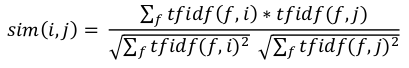
\includegraphics[width=0.5\textwidth]{images/knn_items}

		\subsection{Algoritmos no personalizados}
		Estos algoritmos recomiendan items sin conocer ningún dato del usuario, de forma impersonal como su propio nombre indica. 

		\textbf{Popularidad:} Recomienda los ítems por orden de popularidad y, por tanto, da exactamente el mismo ránking a cada uno de los usuarios. Por popularidad de un ítem se entiende el número de usuarios que han interactuado con el ítem en el sistema. Este método puede parecer trivial, pero es sin embargo uno de los más extendidos en escenarios reales.

		\textbf{Random:} Recomienda ítems de manera aleatoria a cada usuario y su precisión está relacionada con la densidad del conjunto de datos. La efectividad de la recomendación aleatoria, medida con una cierta métrica, se puede interpretar como la esperanza del valor de la métrica sobre el conjunto de datos en el que se aplica. \cite{11}

 \section{Bases de datos orientadas a grafos}
	Las bases de datos relacionales han existido por muchas décadas y son la tecnología de base de datos de elección para la mayoría de almacenamientos intensivos de datos y aplicaciones de obtención de datos. La obtención generalmente se logra mediante SQL, un lenguaje declarativo de consultas. Los sistemas de bases de datos relacionales son generalmente eficientes a menos que la información contenga muchas relaciones que requieren la unión de tablas grandes. Recientemente ha habido mucho interés en los almacenes de datos que no utilizan SQL exclusivamente, el llamado movimiento NoSQL. Ejemplos de ello son BigTable de Google y Cassandra de Facebook. \cite{7}

	Los modelos de bases de datos orientados a grafos se pueden caracterizar como aquellos en los que las estructuras de datos para el esquema y los casos se modelan en forma de grafos o generalizaciones de ellos, y la manipulación de datos se expresa mediante operaciones orientadas a grafos. Estos modelos nacieron en los años ochenta y principios de los noventa en paralelo a los modelos orientados a objetos y su influencia se desvaneció poco a poco con la aparición de otros modelos de bases de datos, en particular la geográfica, espacial, semi-estructurada y XML.

	Recientemente, la necesidad de gestionar la información con naturaleza inherente de un grafo ha hecho volver la relevancia de la zona. De hecho, una nueva ola de aplicaciones para bases de datos de grafos surgió con el desarrollo de las redes grandes (por ejemplo, Web, sistemas geográficos, transporte, teléfonos), y familias de redes generadas gracias a la automatización del proceso de recopilación de datos (por ejemplo, redes sociales y biológicas (incluyendo redes metabólicas, redes de interacción entre proteínas, grafos de estructuras químicas, clústers de genes, y mapas genéticos. Los grafos son realmente una de las más útiles estructuras para modelar objetos e interacciones.\cite{8}

	\subsection{Características}
		No hay índices clásicos en las bases de datos basadas en grafos. Por el contrario, cada objeto almacenado es representado por nodos (entidades) y aristas (relaciones). Un nodo es un registro único que tiene al menos una propiedad. Las aristas definen las relaciones entre los nodos y los nodos y sus relaciones tienen a su vez predefinidas conjuntamente propiedades. Los nodos pueden tener múltiples aristas que definen los diferentes tipos de relaciones que tienen con otros nodos.

		Las consultas en las bases de datos orientadas a grafos están diseñadas para empezar en un nodo específico y explorar sus relaciones con otros nodos. Un ejemplo podría ser: ¿Qué libros están leyendo mis amigos que yo aún no haya leído? Es por eso que este tipo de bases de datos están frecuentemente asociadas con motores de recomendación que se usan con frecuencia en aplicaciones sociales y de comercio electrónico.

		A medida que las búsquedas se van haciendo más complejas, el tiempo de procesamiento va aumentando. Es por eso que las bases de datos basadas en grafos aprenden e indexan las relaciones más comunes con el objetivo de acelerar el tiempo de búsqueda. 
		\subsubsection{Ventajas}
		\begin{itemize}
		 \item Rapidez para conectar datos. En las bases de datos relacionales, el frecuente uso de joins hace que las búsquedas sean lentas.
		 \item Sencillez de las consultas.
		 \item Rapidez en el manejo de consultas complejas que implican múltiples niveles de datos relacionados.
		\end{itemize}
		\subsubsection{Desventajas}
		\begin{itemize}
		 \item La búsqueda de nodos en diferentes máquinas puede ralentizar el proceso drásticamente.
		 \item Requiere un cambio conceptual para los desarrolladores, por lo que implica una curva de aprendizaje.
		\end{itemize}\cite{9}


 \section{Application Programming Interface (API)}
 	Una API (siglas de ‘Application Programming Interface’) es un conjunto de reglas (código) y especificaciones que las aplicaciones pueden seguir para comunicarse entre ellas: sirviendo de interfaz entre programas diferentes de la misma manera en que la interfaz de usuario facilita la interacción humano-software.

	Las API pueden servir para comunicarse con el sistema operativo (WinAPI), con bases de datos (DBMS) o con protocolos de comunicaciones (Jabber/XMPP). En los últimos años, por supuesto, se han sumado múltiples redes sociales (Twitter, Facebook, Youtube, Flickr, LinkedIn, etc) y otras plataformas online (Google Maps, WordPress…), lo que ha convertido el social media marketing es algo más sencillo, más rastreable y, por tanto, más rentable.

	Las API son valiosas, ante todo, porque \emph{permiten hacer uso de funciones ya existentes en otro software} (o de la infraestructura ya existente en otras plataformas) para no estar reinventando lo ya existente constantemente, reutilizando así componentes de software (código) cuyo funcionamiento ha sido probado y determinará una parte del nuevo proyecto. En el caso de herramientas propietarias (es decir, que no sean de código abierto), son un modo de hacer saber a los programadores de otras aplicaciones cómo incorporar una funcionalidad concreta sin por ello tener que proporcionar información acerca de cómo se realiza internamente el proceso. \cite{3}

	Eso es cierto incluso para los programas de código abierto. ¿Quién tiene el tiempo para revisar todo el código de la aplicación de otra persona, el cual puede ser terriblemente desordenado, sólo para usar una función? Las API simplifican todo al limitar el acceso fuera de programa a un conjunto específico de características, a menudo suficientes. Se definen claramente exactamente cómo un programa que va a interactuar con el resto del software, ahorrar recursos y enredos legales potencialmente desagradables en el camino. \cite{10}
